\section{Originale Lademethoden}

Natürlich musste die Bleibatterie des \textsc{Detroit}s auch geladen werden. Für das Laden gab es zwei Unterschiedliche Vorgehensweisen, die kurz vorgestellt werden sollen. Anschliessend wird auf das zum \textsc{Detroit} gehörige Ladegerät eingegangen.

\subsection{Laden in einer Garage}
Viele Garagen boten es an, das bei ihnen gekaufte Fahrzeug auch Laden zu lassen. So mussten die Garagen grosse Leistungen in Form von Gleichspannung zur Verfügung stellen. Diese Gleichspannung konnte mittels zweier Arten erzeugt werden:

Ein \textbf{Umformer} ist eine Motor-Generator-Gruppe, die die Umformung von Wechsel- zu Gleichspannung über den Zwischenschritt der mechanischen Energie ermöglicht. Zu diesem Zweck wird ein erster Motor mit Wechselspannung gespeist. Auf der Achse dieses Motors sitzt eine weitere Maschine, die als Generator für Gleichspannung geschaltet ist. Wird diese Gleichspannungsmaschine als fremderregte Maschine ausgeführt, so ist die Spannung ausserdem in ihrem Betrag regelbar.

Alternativ kann die Gleichrichtung auch mit einer \textbf{Quecksilberdampfröhre} erfolgen. Dies ist eine Glasröhre, an deren unteren Ende sich ein See aus flüssigem Quecksilber befindet, der als Kathode fungiert. Über diesem See befindet sich eine Heizwicklung, die zum Start das flüssige Quecksilber erwärmt und damit verdampfen lässt. Kondensiert dieses Quecksilber wieder, so kann es über die Glaswände zurück fliessen. Am oberen Ende der Glasröhre befindet sich eine Anode. Um das weitere Funktionsprinzip zu verstehen muss ausserdem bekannt sein, dass sich die Elektronen sehr einfach aus dem Quecksilberdampf lösen können.

Nun sollen damit die beiden Spannungsrichtungen, die sich bei Wechselspannung mit der Netzfrequenz abwechseln, untersucht werden. Ist die Spannung von der Anode zur Kathode positiv, so werden die aus dem Quecksilberdampf gelösten Elektronen in Richtung der Anode beschleunigt und ein Stromfluss kommt zustande. Ist die Spannung zwischen Anode und Kathode hingegen negativ, so werden die gelösten Elektronen wieder zurück in den Quecksilbersee gezogen. Es fliesst also kein Strom zwischen Anode und Kathode. Da der Strom also nur während einer Spannungspolarität fliessen kann, steht am Ende eine \textcolor{blue}{pulsierende} Gleichspannung zur Verfügung.

Bei Privatfahrzeugen wurden die Batterien meist geladen, während sie sich im Auto befanden. Dazu wurden vom zentralen Gleichrichter Leitungen zu den einzelnen Ladestationen verlegt, bei welchen der Strom indirekt mittels eines stufenlosen Lastwiderstandes (eines sogenannten Rheostaten) reguliert werden konnte. Gerade bei Taxis oder Lastwagen war es aber auch weit verbreitet, die Batterien aus dem Fahrzeug zu entnehmen und in einem sogenannten "`Batterieraum"' zu laden. Das Fahrzeug konnte während dieser Zeit mit einem anderen Satz Batterien weiter benutzt werden. Beide Vorgehen sind in den Abbildungen \ref{fig:Laden_Garage} und \ref{fig:Laden_Batterieraum} auf der folgenden Seite gezeigt.

\begin{landscape}
\begin{figure}
\begin{minipage}{0.65\textwidth}
	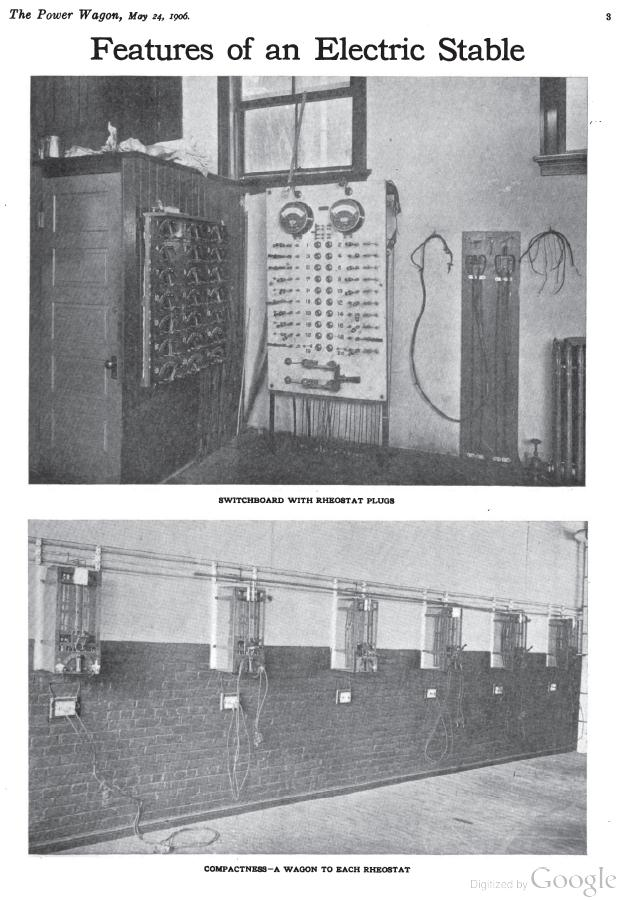
\includegraphics[width=\textwidth]{images/Laden_Garage.jpg}
	\caption{Ladestation für mehrere Fahrzeuge \cite{laden_alt}}
	\label{fig:Laden_Garage}
\end{minipage}
\begin{minipage}{0.65\textwidth}
	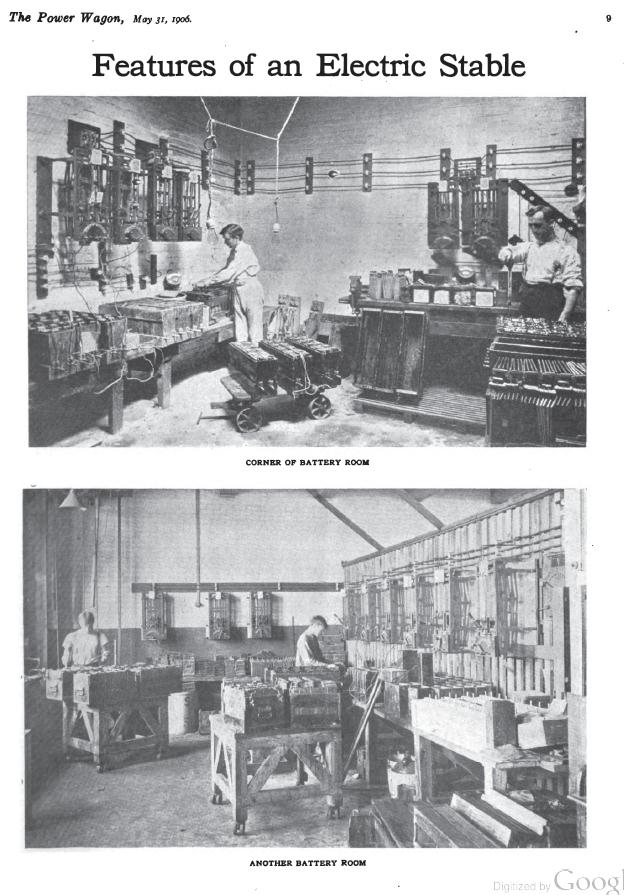
\includegraphics[width=\textwidth]{images/Laden_Batterieraum.jpg}
	\caption{Laden der Batterien in einem Batterieraum \cite{laden_alt}}
	\label{fig:Laden_Batterieraum}
\end{minipage}
\end{figure}
\end{landscape}

\subsection{Laden des Fahrzeuges zuhause}
Für das Laden zuhause gibt es ein dem \textsc{Detroit} zugehöriges Ladegerät. Das hier untersuchte Modell "`Burtoni \& Rogers Junior Twin Six 12 Hour Charger"' besitzt die folgenden Daten:

\begin{tabular}{lll}
	\textbf{Originalbezeichnung} & \textbf{---\quad Deutsche Bezeichnung:} & \textbf{Wert} \\
	Volts A.C. & ---\quad Wechselspannung Eingangsseitig: & $110$ V (US-amerikanisches Netz) \\
	Cycles & ---\quad Netzfrequenz: & $60$ Hz (US-amerikanisches Netz)\\
	Amps A.C. & ---\quad Wechselstrom Eingangsseitig: & $12$ A \\
	Watts A.C. & ---\quad Leistung Eingangsseitig: & $1050$ W \\
	Volts D.C. & ---\quad Gleichspannung Ausgangsseitig: & $60$ V \\
	Amps D.C. & ---\quad Gleichstrom Ausgangsseitig: & $12$ A \\
	Model & ---\quad Modelltyp: & JR-3 \\
	Ser. & ---\quad Seriennummer: & 19759
\end{tabular}

Wie man auf den ersten Blick erkennt, ist der Strom auf der Ein- und der Ausgangsseite der selbe. Das lässt darauf schliessen, dass sich dazwischen kein Transformator befindet. Durch einen ersten Gedanken zur Funktion resultierte also das in Abbildung \ref{fig:Ladegeraet1} gezeigte Schema:

\begin{figure}[h]
	\centering
		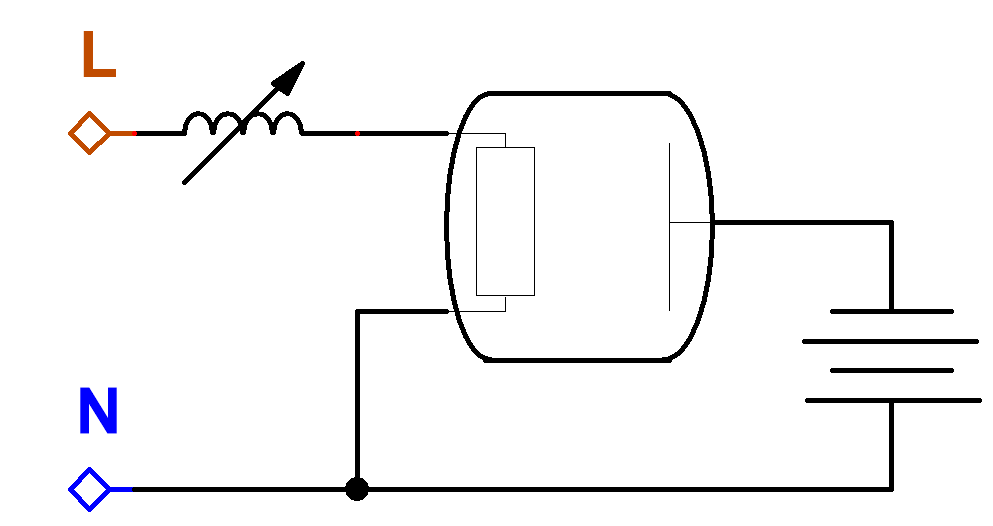
\includegraphics[width=0.60\textwidth]{images/Ladegeraet_Alt_1.PNG}
	\caption{Röhrengleichrichter mit einer Heizspannung von $230$ VAC}
	\label{fig:Ladegeraet1}
\end{figure}

Dabei wird zuerst der Stromfluss durch eine veränderbare Induktivität begrenzt. Eine anschliessende Gleichrichterröhre, deren Funktion noch erklärt wird, sorgt dafür, dass nur die Halbwelle der gewünschten Polarität durchgeleitet wird. Dieser begrenzte Gleichstrom kann nun zum Laden der Batterie verwendet werden.

Die verwendete Gleichrichterröhre funktioniert dabei anders als die bereits vorgestellten Quecksilberdampfgleichrichter. In Gleichrichterröhren befindet sich ein Glühdraht, welcher gleichzeitig auch als Kathode fungiert. Dieser Glühdraht wird mittels einer Spannung beheizt, zusätzlich liegt an einem Ende das Kathodenpotential an. Durch die hohe Temperatur wird auch hier das Lösen von Elektronen ermöglicht, welche bei richtiger Spannungspolarität der Anoden-Kathodenspannung zur Anode beschleunigt werden. Da lediglich eine Halbwelle durchgeleitet wird, ist auch hier eine Gleichrichtung erfolgt. Eine der beiden im Ladegerät verbauten Gleichrichterröhren ist in Abbildung \ref{fig:Roehre_Diode} gezeigt: \newpage

\begin{figure}[h]
	\centering
		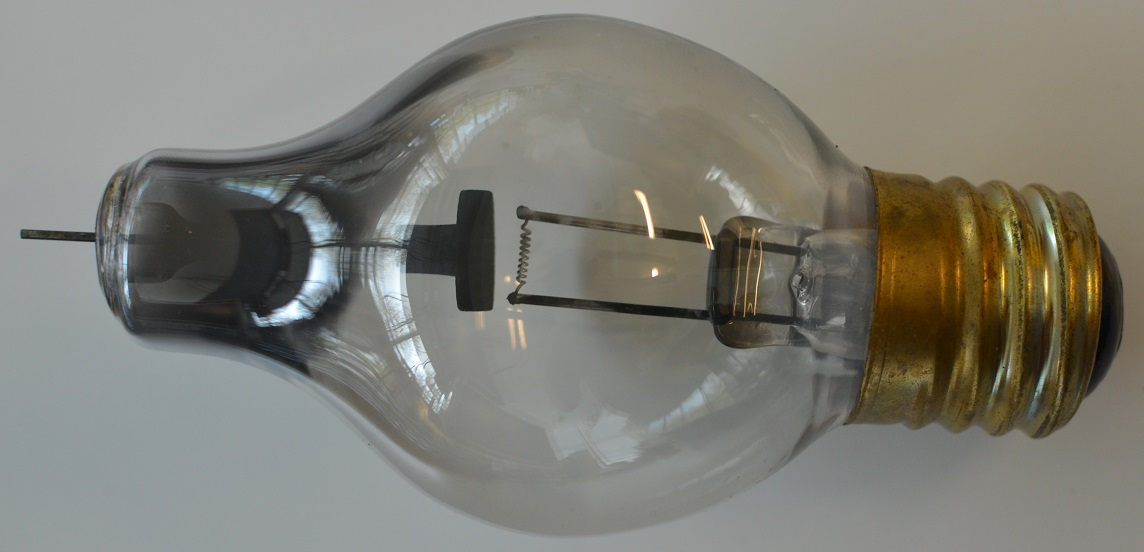
\includegraphics[width=0.75\textwidth]{images/Roehre_Diode.jpg}
	\caption{Gleichrichterröhre, auch Diode genannt}
	\label{fig:Roehre_Diode}
\end{figure}

Es konnte jedoch schnell gezeigt werden, dass dies nicht die im Ladegerät verbaute Schaltung ist. So ist zum einen auf dem Gehäuse die Bezeichnung "`Balanced Full Wave"' angebracht, was darauf hindeutet, dass beide Halbwellen gleichgerichtet werden. Zum anderen ist eine Anzeige vorhanden, mit der überwacht wird, dass beide Röhren gleich belastet werden. Dies ist ein Hinweis darauf, dass beide Röhren nicht einfach nur parallel geschaltet sind, sondern sie je eine Halbwelle gleichrichten und bei ungleichmässigen Strömen das Eisen des Transformators asymmetrisch belastet wird. Aus diesen Überlegungen konnte die Schaltung des Netzgerätes hergeleitet werden und ist in Abbildung \ref{fig:Schema_Ladegeraet_Alt} gezeigt, es handelt sich dabei um eine sogenannte Mittelpunktschaltung:

\begin{figure}[h]
	\centering
		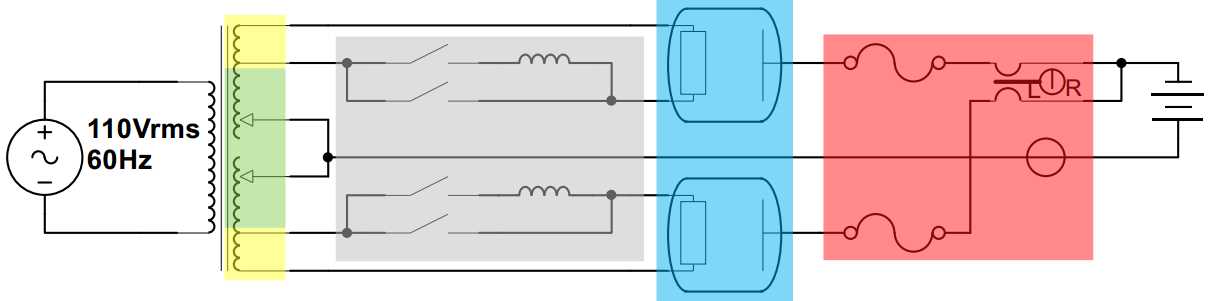
\includegraphics[width=1.00\textwidth]{images/Ladegeraet_Alt_2.PNG}
	\caption{Schaltung des originalen Netzgerätes}
	\label{fig:Schema_Ladegeraet_Alt}
\end{figure}

Es soll an dieser Stelle noch kurz die Funktion des Ladegerätes vorgestellt werden. Begonnen wird dabei mit der eingangsseitigen Transformatorenwicklung. Diese sorgt dafür, dass sämtliche Wicklungen auf der Sekundärseite ebenfalls Spannung abgeben können. Die ersten beiden dieser Wicklungen sind die gelb hinterlegten Heizwicklungen. Diese sorgen dafür, dass die Heizwicklungen, die ja möglichst niederohmig sein sollen (um den gleichzurichtenden Stromfluss nicht zu bremsen), mit einer niedrigen Spannung versorgt werden können. Über die beiden grün gefärbten Transformatorenwicklungen lässt sich die Höhe der ausgangsseitigen Gleichspannung und damit am Ende auch der Gleichstrom regulieren. Dies geschieht über den Drehknopf, welcher sich mittig an der Front des Ladegerätes befindet.

\newpage

Der graue Bereich wird vom Schalter beeinflusst, welcher sich rechts an der Front befindet. So sind in der Aus-Stellung beide Schalter geöffnet, sodass keine Verbindung zur Batterie besteht. Bei Stufe eins von zwei wird der Stromfluss durch die Induktivität zusätzlich behindert, was in kleineren Strömen im Vergleich zu Stufe zwei resultiert, bei welcher die Induktivität überbrückt wird. Die Funktion der beiden Gleichrichterröhren wurde bereits erläutert. Sie sorgen dafür, dass jeweils nur eine Halbwelle durchgeleitet wird (die positive Halbwelle bei der unteren Röhre und die negative Halbwelle bei der oberen Röhre). Durch die Kombination der beiden Halbwellen erhält man eine pulsierende Gleichspannung, welche beide Halbwellen gleichrichtet.

Es folgen noch die rot hinterlegten Sicherheits- und Überwachungsbauteile. Die beiden Sicherungen sorgen dafür, dass kein übermässiger Strom zu den Batterien fliessen kann. Das Amperemeter zeigt den aktuellen Stromfluss an, sodass eventuell mit dem Transformator nachgeregelt werden kann. Interessant sind die beiden gekoppelten Spulen. Dazu werden die Anodenleitungen beider Röhren durch einen gemeinsamen Eisenkern geführt. Sind die Stromflüsse in beiden Röhren gleich, so wird keine Spannung induziert beziehungsweise ist deren Frequenz zu hoch, um das mechanische Anzeigegerät auszulenken. Ist der Stromfluss hingegen asymmetrisch, so wird eine Spannung induziert und dies auf dem Messgerät angezeigt. Dadurch wird darauf hingewiesen, dass der Transformator einseitig belastet wird.

Abschliessend soll noch ein Blick in das originale Ladegerät geworfen werden (siehe Abbildung \ref{fig:Ladegeraet_Original}). Sehr gut erkennt man den grossen Transformator in der Mitte mit den vielen Abgriffen, die beiden Röhrensockel rechts und links sowie darunterliegend die überbrückbaren Drosselspulen:

\begin{figure}[h]
	\centering
		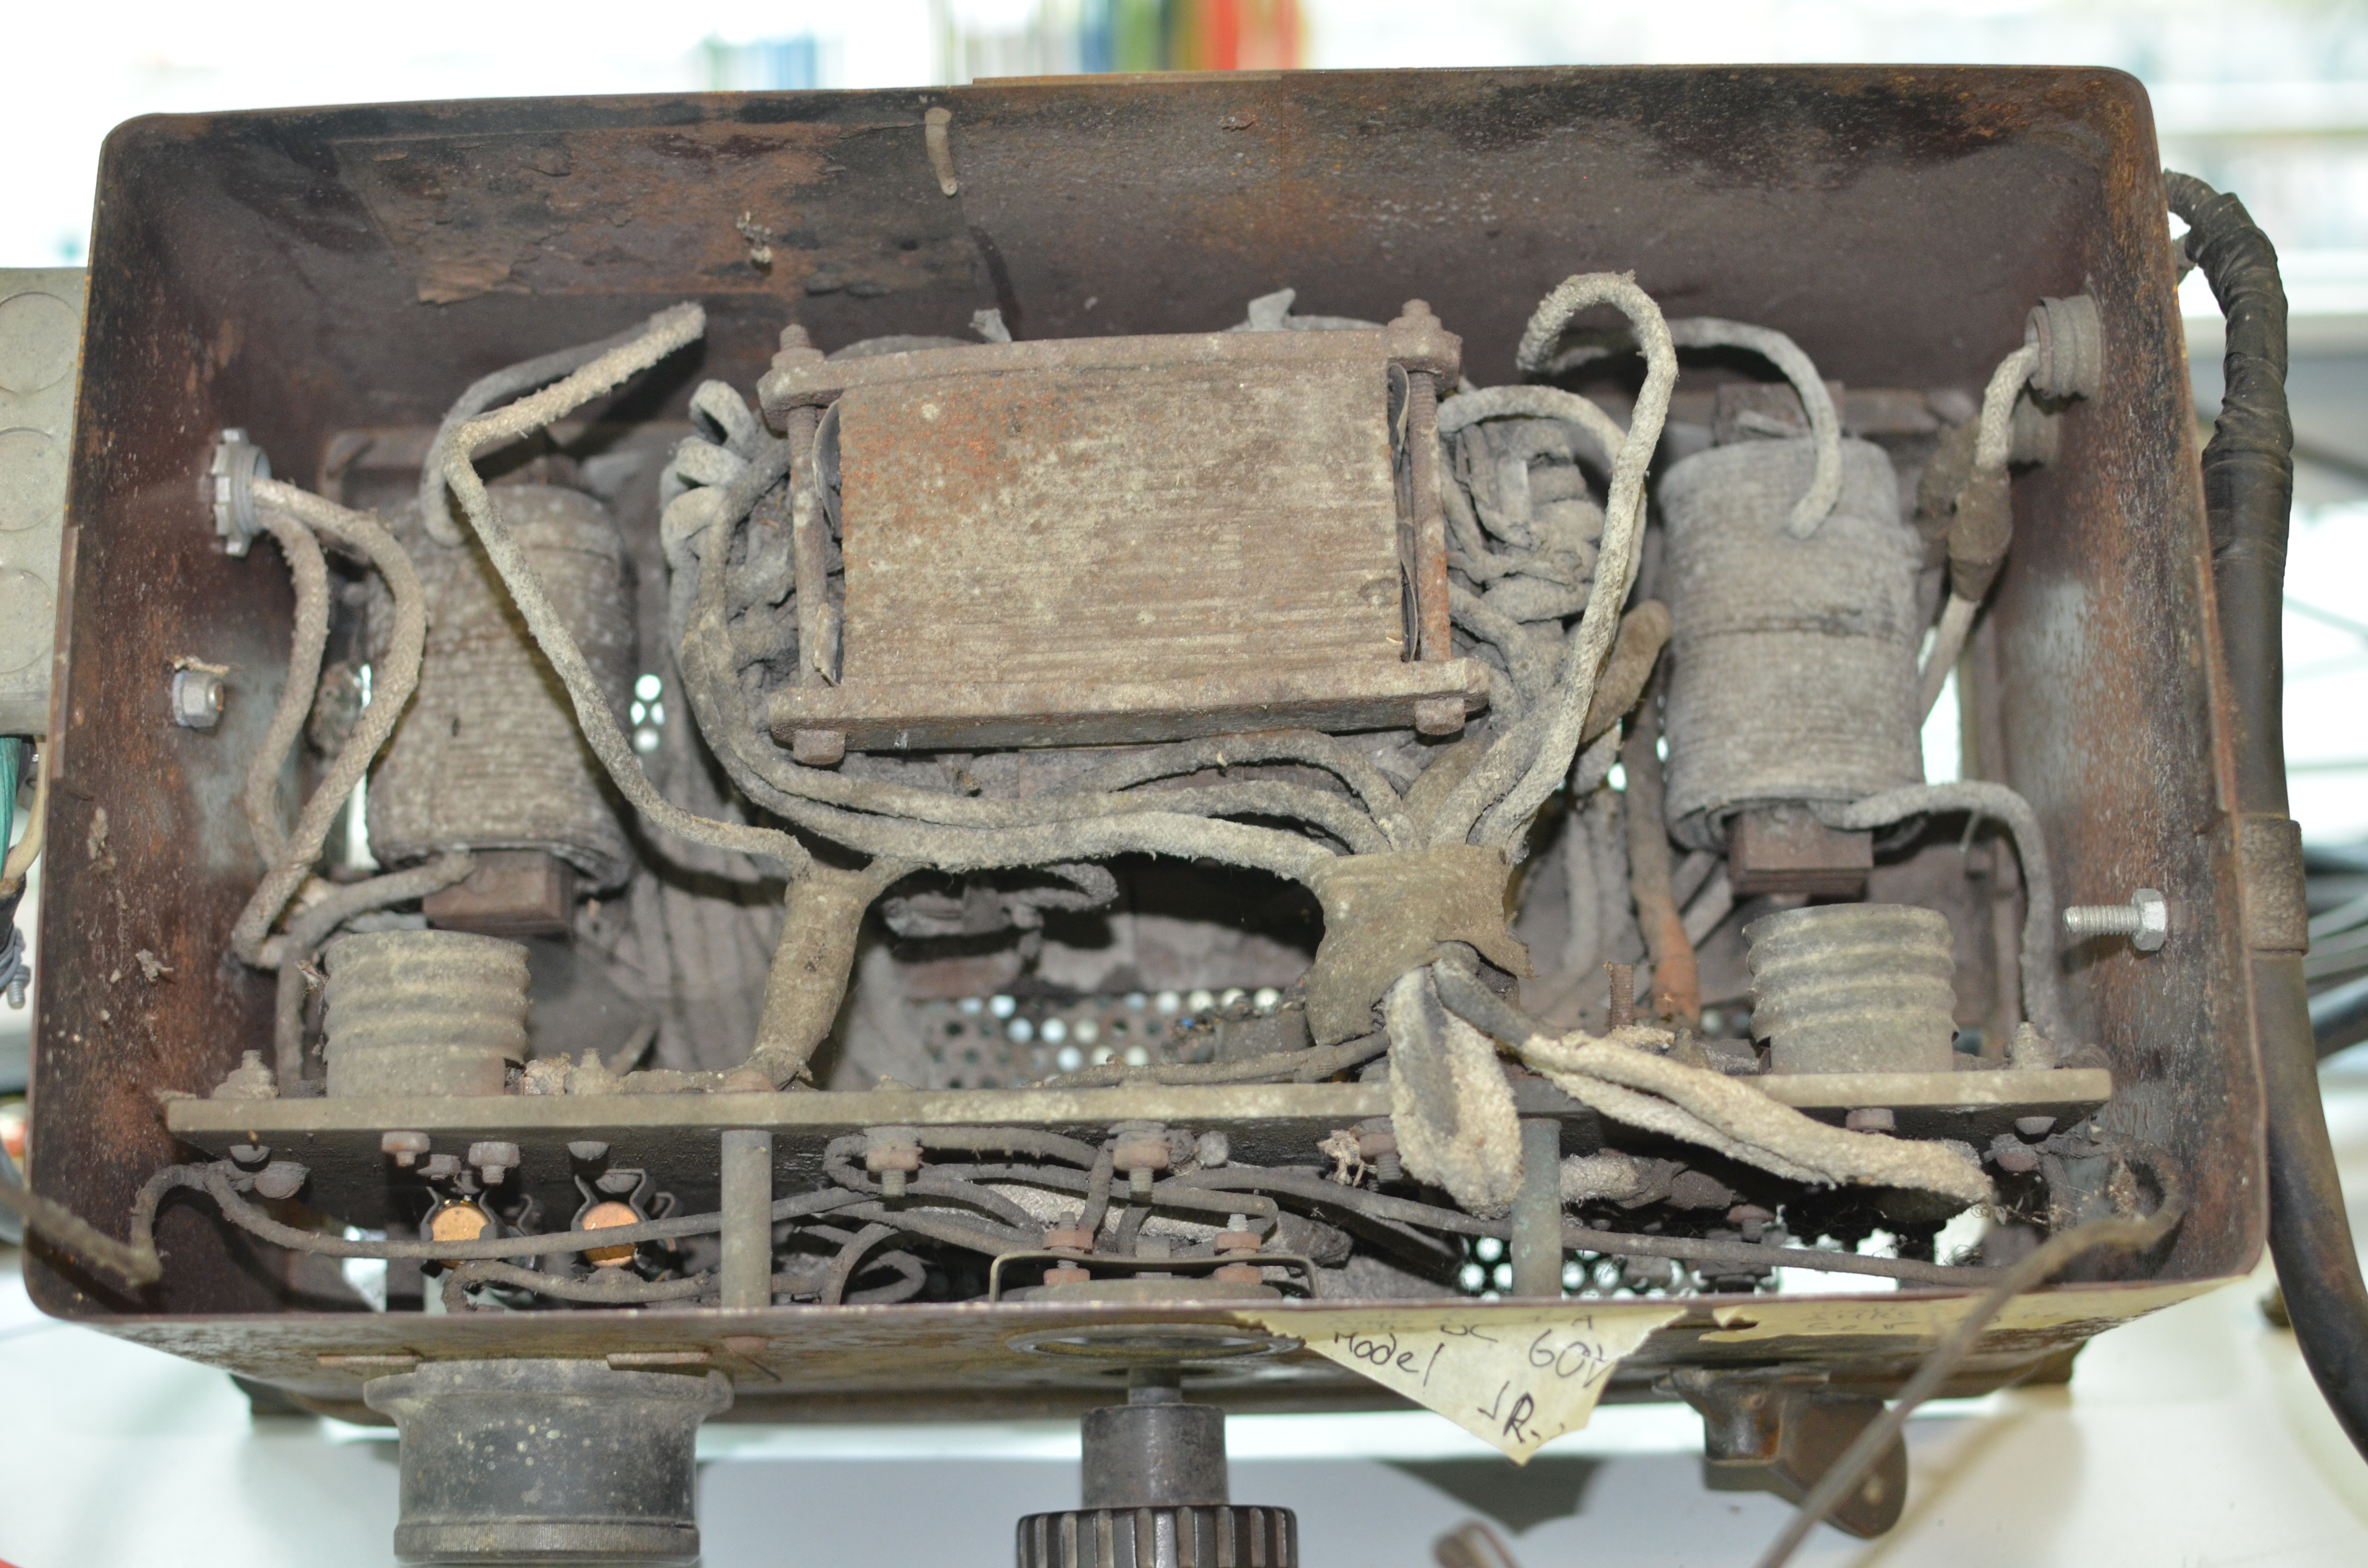
\includegraphics[width=0.95\textwidth]{images/Ladegeraet_Original.JPG}
	\caption{Das geöffnete originale Ladegerät von Oben betrachtet (1: Transformator, 2: Drosselspule, 3: Sockel für Gleichrichterröhren, 4: Umschalter Ladestufe, 5: Spannungsregelung Transformator, 6: Symmetrieüberwachung, 7:Amperemeter)}
	\label{fig:Ladegeraet_Original}
\end{figure}

\newpage